\documentclass[../report.tex]{subfiles}
\begin{document}
\subsection{Nguyên lý hoạt động của Module 4 led đơn  7 thanh}
\subsubsection{Led 7 thanh đơn}
\begin{itemize}
    \item Led 7 thanh đơn được chia làm 2 loại: Led a-nốt chung và Led ca-tốt chung
    \begin{figure}[H]
        \centering
        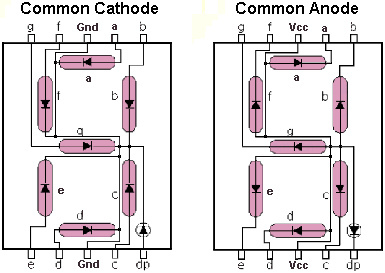
\includegraphics[width=9cm]{figures/led7.jpg}
        \caption{Led 7 đoạn ca-tốt chung (trái) và a-nốt chung (phải)}
    \end{figure} 
    
    \item Cả hai loại này có đều có cấu tạo từ 8 con led đơn ghép lại với nhau thành hình số 8 và 1 dấu chấm:
    \begin{figure}[H]
        \centering
        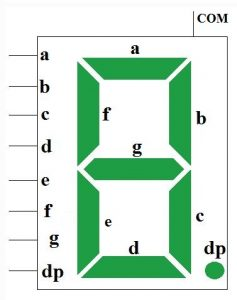
\includegraphics[width=9cm]{figures/ledS.jpg}
        \caption{Cấu trúc Led 7 thanh đơn}
    \end{figure} 

    \item Cấu tạo led 7 thanh:
        \begin{itemize}
            \item 8 chân dương của 8 led đơn sẽ được nối chung với nhau ( vào chân COM).
            \item Các chân âm sẽ được nối ra làm các chân dữ liệu a, b, c, d, e, f, g, dp.
            \item Để diều khiển led 7 thanh anode chung, ta phải cấp nguồn dương và cổng COM và xuất dữ liệu tích cực ở mức 0 ra 8 chân dữ liệu để hiện thị theo ý muốn. 
        \end{itemize}
    \item Led 7 thanh chung katot thì ngược lại.

    \item Bảng mã led 7 thanh giả sử led 7 thanh trong sơ đồ thiết kế mạch là loại led 7 thanh chung anode. Các chân a, b, c,d, e, f, g, dp lần lượt được nối vào các chân P0.0 đến P0.7 của cổng P0.
	Để hiện thị các số từ 0 đến 9 thì dữ liệu xuất ra ở cổng P0 phải có dạng mã hexa như sau:
            \begin{center}
                    \begin{tabular}{ |c|c|c|c|c|c|c|c|c|c|c| } 
                    \hline
                    Số & 0 & 1 & 2 & 3 & 4 & 5 & 6 & 7 & 8 & 9  \\
                    \hline
                    Mã Hexa Led 7 CA & 0xC0 & 0xF9 & 0xA4 & 0xB0 & 0x99 & 0x92 & 0x82 & 0x8F & 0x80 & 0x90\\ 
                    \hline
                    \end{tabular}
                    
            \end{center}
\end{itemize}

\subsubsection{Module 4 led đơn  7 thanh}
\paragraph*{}Module 4 Led 7 thanh trong hệ thống là Module 4 led 7 thanh chung anode. 4 chân COM của 4 led được nối với các cổng P1.0 đến P1.3 thông qua 1 con node. các led 7 thanh đơn sẽ được “on” khi đầu vào các chân COM của nó ở mức 0, và “off” khi là 1. 
8 chân dữ liệu a, b, c,d, e, f, g, dp của mỗi led được nối vào các chân P0.0 đến P0.7 của cổng P0.

\subsubsection{Thuật toán quét led}
\begin{enumerate}
    \item Hiển thị LED0
        \begin{enumerate}
            \item Đặt dữ liệu của LED0 ra P0
            \item Đặt P1.0 = 0 (bật LED 0)
            \item Trễ n ms
            \item Đặt P1.0 = 1 (tắt LED 0)
        \end{enumerate}
    
    \item Tiếp tục hiển thị các LED còn lại
    \item Quay vòng về LED0
\end{enumerate}

\subsection{Xử lý ngắt trong vi điều khiển AT89S52}
\begin{itemize}
    \item Vi điều khiển AT89S52 thuộc họ 8051 có tất cả 5 ngắt và 1 ngắt Reset và 2 bộ định thời Timer0 và Timer1.
    \item Ngắt reset là ngắt phần cứng khi ta kích mức cao vào chân Reset
    \item 5 ngắt còn lại bao  gồm: Ngắt Timer0, Timer 1, Ngắt ngoài 0, Ngắt ngoài 1, Ngắt UART
    \item Ngắt timer : Ta xét thanh ghi hoạt động của timer: Thanh ghi 8bit TMOD:
        \begin{center}
                    \begin{tabular}{ |c|c|c|c|c|c|c|c| } 
                    \hline
                    GATE & C/T & M1 & M0 & GATE & C/T & M1 & M0 \\
                    \hline
                    \end{tabular}
        \end{center}
        \begin{itemize}
            \item 4 bit cao của Thanh ghi TMOD là dùng để set chế độ cho timer1, 4 bít thấp dùng để sét chế độ cho timer0, nhưng ta chỉ quan tâm đến 2 bit M1 và M0:
            \begin{center}
                    \begin{tabular}{ |c|c|c|c| } 
                    \hline
                    M1 & M0 & Chế độ & Chế độ hoạt động \\
                    \hline
                    0 & 0 & 0 & Định thời 13 bit \\
                    0 & 1 & 1 & Định thời 16 bit \\
                    1 & 0 & 2 & Định thời 8 bit và tự nạp lại \\
                    1 & 1 & 3 & Định thời chia tách \\
                    \hline
                    \end{tabular}
                    
            \end{center}

            Giả sử khi chúng ta khai báo TMOD = 0x11 tức là 0001 0001 $\rightarrow$ set timer 0 và timer1 đều ở chế độ định thời 16 bit
            \item Thanh ghi TH0, TL0(timer0), TH1,TL1(timer1) nạp giá trị ban đầu để đếm, bộ định thời sẽ đếm lên 1 với mỗi chu kì máy, như vậy ta phải tính toán giá trị nạp vì khi bộ định thời tràn tức đã đếm đủ 8bit, 16bit thì ngắt mới xảy ra. Chú ý thanh ghi TH0, TH1 có tác dụng khi ở chế độ 16bit vì nó lưu 8bit cao.
            \item Thanh ghi IE(thanh ghi khai báo ngắt) có 2 bit ET0 và ET1 tương ứng ngắt timer0 và ngắt timer1. ví dụ khai báo ET0=1 cho phép ngắt timer0
            \item Thanh TR0, TR1 để cho phép timer0 và timer1 bắt đầu đếm. Ví dụ TR0 =1 cho phép timer0 chạy. TR0 =0 dừng timer0
        \end{itemize}

    \item Ngắt ngoài:
        \begin{itemize}
            \item Để sử dụng ngắt ngoài ta cần phải kết nối vào 2 chân cho phép ngăt là P3.2(INT0) và P3.3(INT1)
            \item Thanh ghi ngắt IE có 2 bit EX0 và EX1 tương ứng với chọn ngắt ngoài 0 hay ngắt ngoài 1. Ví dụ : EX0 =1 cho phép ngắt ngoài 0
        \end{itemize}

    \item Bảng Vector ngắt:
        \begin{center}
                    \begin{tabular}{ |c|c|c|} 
                    \hline
                    Ngắt & Địa chỉ ROM(Hexa) & Chân\\
                    \hline
                    RESET & 0000 & 9 \\
                    Ngắt ngoài 0(INT0) & 0003 & 12 (P3.2) \\
                    Ngắt Timer 0(TF0) & 000B & \\
                    Ngắt ngoài 1(INT1) & 0013 & 13 (P3.3) \\ 
                    Ngắt Timer 0(TF0) & 001B & \\
                    Ngắt COM nối tiếp (RI và TI) & 0023 & \\
                    \hline
                    \end{tabular}
                    
        \end{center}
        
    
    \item Thanh ghi ưu tiên ngắt ( IP)
        \begin{center}
                    \begin{tabular}{ |c|c|c|c| } 
                    \hline
                    Bit & Ký hiệu & Địa chỉ bit &  Mô tả (1: mức cao, 0: mức thấp) \\
                    \hline
                    IP.7 & - & - & Không sử dụng \\
                    IP.6 & - & - & Không sử dụng \\
                    IP.5 & PT2 & 0BDh & Ưu tiên ngắt do bộ định thời 2 \\
                    IP.4 & PS & 0BCh & Ưu tiên ngắt do port nối tiếp \\                
                    IP.3 & PT1 & 0BBh & Ưu tiên ngắt do bộ định thời 1 \\                    
                    IP.2 & PX1 & 0BAh & Ưu tiên ngắt ngoài 1 \\
                    IP.1 & PT0 & 0B9h & Ưu tiên ngắt do bộ định thời 0\\
                    IP.0 & PX0 & 0B8h & Ưu tiên ngắt ngoài 0 \\
                    \hline
                    \end{tabular}
                    
        \end{center}

        Ví dụ khi khởi tạo IP= 0x0A = 0000 1010 $\rightarrow$ độ Ưu tiên ngắt timer1, và timer0 cao hơn ngắt ngoài 0 và 1
        \begin{itemize}
            \item Khi 2 ngắt đến đồng thời thì ngắt nào có độ ưu tiên cao hơn sẽ được thực hiện trước
            \item Khi 2 ngắt cùng mức ưu tiên xuất hiện thì các ngắt sẽ được thực hiện lần lượt theo chuỗi vòng sau: 
            		Ngắt ngoài 0 > ngắt timer0 > ngắt ngoài 1 > ngắt timer1 > ngắt UART.
        \end{itemize}
        
\end{itemize}

\subsection{Lập trình tạo độ trễ cho timer}
\begin{itemize}
    \item Giả sử Tần số đồng hồ của bộ định thời = 1/12 tần sô dao động của bộ dao động  thạch anh
    \item Giả sử tần số của thạch anh là 12MHz $\rightarrow$ tần số bộ định thời là 1 MHz $\rightarrow$ chu kì của bộ định thời là T = 1us. $\rightarrow$ cứ 1us thì bộ định thời sẽ đếm lên 1 chu kì máy hay giá trị 16 bít lưu ở thanh ghi TH( 8 bit cao, TL( 8 bít thấp) sẽ tăng lên 1. Với chế độ 1, thì khi giá trị 16 bit lưu ở 2 thanh ghi TH và TL lớn hơn $2^16$ = 65536 $\rightarrow$ xảy ra ngắt timer
    \item Nếu giả sử cần tạo 1 độ trễ d  = 50 ms = 50,000.T$\rightarrow$ cần thiết lập giá trị 16 bit ban đầu lưu ở 2 thanh ghi TH và TL là 65536-50000= 15536 = 3cb0 ở dạng hex. $\rightarrow$ cần gán TH = 0x3c, TL = 0xb0
    \item Xét chương trình:
        \begin{figure}[H]
            \centering
            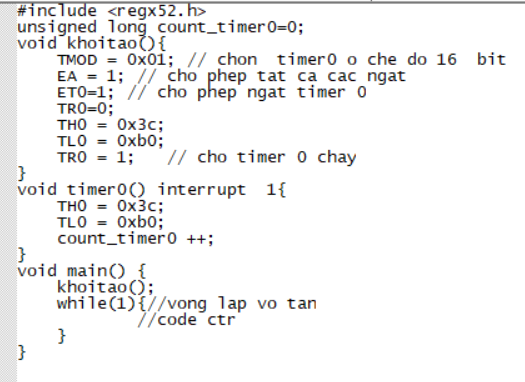
\includegraphics[width=9cm]{figures/code.png}
        \end{figure} 
    
        Ta thấy ở hàm khoitao(), ta gán giá trị cho 2 thanh ghi TH0 = 0x3c, và Tl0= 0xb0 $\rightarrow$ tức là giá trị ban đầu là 15536, sau 50000 chu kì máy hay 50 ms xảy ra hiện tượng tràn bít, thanh ghi TF được set là 1, hàm ngắt timer 0 được gọi$\rightarrow$ biến count\_timer0 tăng lên 1
$\rightarrow$ cứ 50ms biến count\_timer0 lại được tăng lên 1
$\rightarrow$ 1s có 20 lần biên count\_time0 được tăng lên 1
$\rightarrow$ thời gian từ lúc chạy chương trình đến lúc hiện tại = count\_timer0/20

\end{itemize}

\subsection{Lập trình phát nhạc ra loa}
\paragraph*{}Giả sử muốn phát 1 ra loa 1 tần số f = 250Hz  tương ứng vs chu kì  là 1/250 = 4ms. Ta làm như sau:
    \begin{itemize}
        \item  Giả sử Loa được nối với chân P1.5 của Vi điều khiển.  Tần sô thạch anh là 12Mhz $\rightarrow$ tần sô bộ định thời 1Mhz, chu kì bộ định thời To = 1us. Timer0 được set ở chế độ 16 bit
        \item  Chu kì tần sô âm muốn phát ra T= 4ms = 4000To $\rightarrow$ khoảng cách  2 lần phát màng loa ở biên âm và biên dương ( nửa chu kì ) là 2ms = 2000To $\rightarrow$ cần set gia trị cho thanh ghi TH0 và TL0 1 giá trị 16 bit = 65536-2000= 63536 = 0xf830$\rightarrow$ TH0= 0xf8, TL0=0x30

    \end{itemize}

\subsection{Phân biệt bấm nút chế độ long-press và short-press}
Dựa vào khoảng thời gian kể từ lúc nhấn đến lúc nhả ra để xác định xem đó là long-press hay short-press. Nếu khoảng thời gian đó lớn hơn 1s thì đó là long-press, ngược lại là short-press


\end{document}
